\documentclass{report}
\usepackage{tikz} % package principal TikZ
\usepackage{pgfplots}
\pgfplotsset{width=12cm,compat=newest}
 
%------------------
\begin{document}
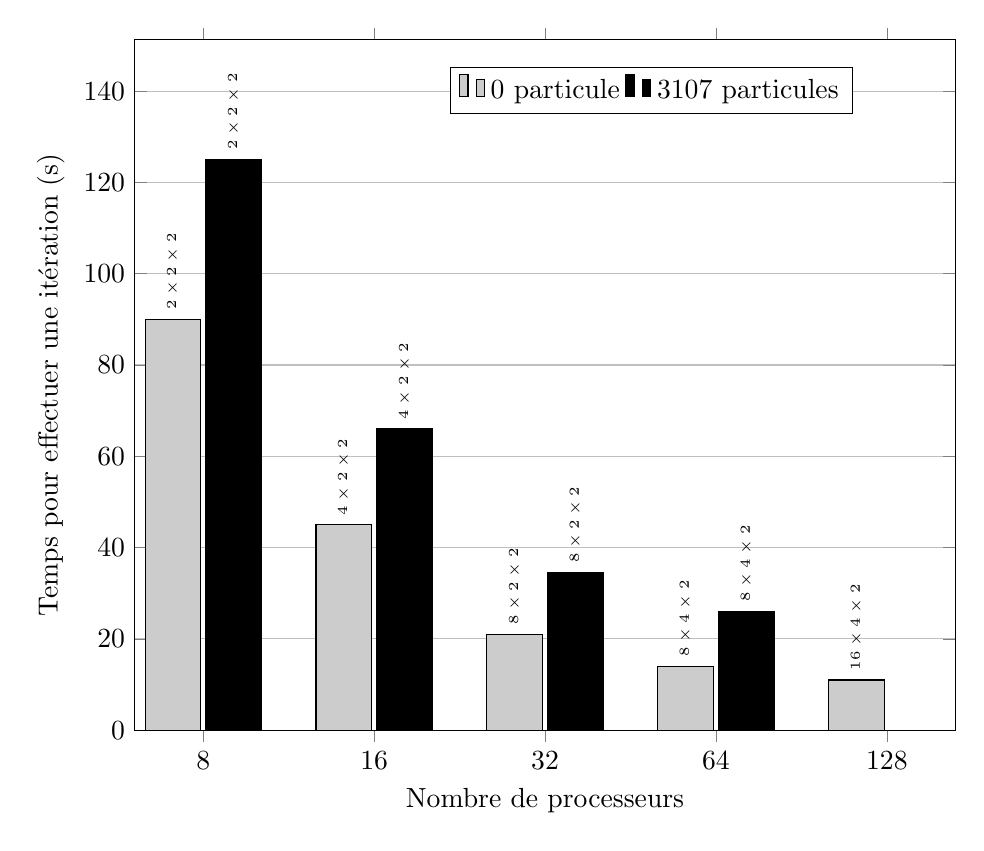
\begin{tikzpicture} \begin{axis}[
    x tick label style={
        /pgf/number format/1000 sep=},
    ymajorgrids,
    ylabel=Temps pour effectuer une it\'eration (s),
    xlabel= Nombre de processeurs,
    nodes near coords,
    point meta=explicit symbolic,
    xtick={1,2,3,4,5},
    xticklabels={$8$,$16$,$32$,$64$,$128$},
    enlarge y limits={upper,value=0.21},
    legend style={at={(0.63,0.96)},
        anchor=north,legend columns=-1},
    ybar,
    every node near coord/.append style={rotate=90, anchor=west,font=\tiny},
    bar width=20pt,
]
\addplot [ybar,fill=gray!40]
    coordinates {(1,90)[$2\times2\times2$] (2,45)[$4\times2\times2$]
         (3,21)[$8\times2\times2$] (4,14)[$8\times4\times2$] (5,11)[$16\times4\times2$]};
\addplot [ybar,fill=black]
    coordinates {(1,125)[$2\times2\times2$] (2,66)[$4\times2\times2$]
        (3,34.5)[$8\times2\times2$] (4,26)[$8\times4\times2$] (5,0)[$\varnothing$]};
\legend{0 particule,3107 particules,temps th\'eorique}
\end{axis}
\end{tikzpicture}
\end{document}
